This section describes our approach to specifying and updating robot missions taking place in open worlds. 
Our presentation takes the form of requirements on a specification language $\Lambda$, such that mission specifications $\mathcal{M}(AP) \in \Lambda$, parsed by $\mathcal{P}_{\Lambda}$ satisfy Eqs. \eqref{Eq:newSpecA} and \eqref{Eq:newSpecB}. 

First, we leverage the expressive power of open-world abstraction to specify high-level behaviors without referring to individual propositions $\pi \in AP_k$. 
Then, we show that the addition of new propositions to a mission specification $\mathcal{M}_k = \mathcal{M}(AP_k)$ has to follow certain rules, such that correspondence $\mathcal{C}: AP \rightarrow 2^{AP}$ between groups of propositions is maintained, where $2^{AP}$ denotes the power set of $AP$.
Finally, we provide a mechanism that allows the user to explicitly specify when the updated specification $\mathcal{M}_{k+1} = \mathcal{M}(AP_{k+1})$, and consequently the GR(1) formula 
%$\varphi [k+1] = \mathcal{P}_{\Lambda} (\mathcal{M}_{k+1}, AP_{k+1})$, 
$\varphi [k+1] = \mathcal{P}_{\Lambda} (\mathcal{M}_{k+1})$,
should be synthesized into a revised robot controller.

\subsection{Defining Tasks over Open Worlds}

The first requirement on specifications $\mathcal{M}_0 = \mathcal{M}(AP_0) \in \Lambda$ is the definition of groups of propositions $G_i$ and the definition of correspondence, $\mathcal{C}$, between groups of propositions. Then, tasks that refer to individual propositions $\pi \in G_i$ can be replaced by tasks over $G_i$ and $G_j \in \mathcal{C}(G_i), \; j \not = i$. The superscript $i$ will often be omitted for clarity of notation.

An advantage of open-world abstractions is the ability to specify a mission even if the groups contain no propositions prior to execution, i.e., $G_i = \emptyset$, $G_i \in \mathcal{M}_0$. In this case, the groups will be populated on-the-fly as new elements in the world are discovered (see Section \ref{rewriting}, and Examples \ref{Ex:SnS}, \ref{Ex:mailbot3}).

\begin{myExample}\label{Ex:mailbot2}We revisit Example \ref{Ex:mailbot1} and make use of the open world abstractions. For illustrative purposes, we use Structured English \cite{JFRKGICRA12} as the specification language $\Lambda$.
\begin{algorithm}
\textbf{Mission specification:} (partial) Autonomous Mailbot
	
	\vspace{-6 pt}
	\hrulefill\\
	{\small
\texttt{1: Group Letters is letter1, letter2} \\
\texttt{2: Group Offices is office1, office2} \\
\texttt{3: Letters correspond to Offices} \\
\texttt{4: If you are sensing any Letter then}\\
\texttt{go to the corresponding Office}\\ 
}
\vspace{-10 pt}
\end{algorithm}

Let $G_1$ be \texttt{Letters} and $G_2$ be \texttt{Offices}. Line 3 establishes correspondence from $G_1$ to $G_2$, .i.e., $G_2 \in \mathcal{C}(G_1)$. We use the notation $G_2 \in \mathcal{C}(G_1)$, rather than $G_2 = \mathcal{C}(G_1)$, because $G_1$ could potentially correspond to more groups, e.g. $\mathcal{C}(G_1) = \left\{ G_2, G_3, \ldots\right\}$. 
Notice how the task in line 4 does not refer to any particular letters or offices. 
As already mentioned, even if $G_1, G_2 \in \mathcal{M}_0$ were empty, the user would still be able to specify the mission above.
%In the special case where $G_j^i = \mathcal{C}(G_i)$, we can drop the superscript $i$, and write $G_j$, as in this example.
\end{myExample}

Let a letter corresponding to a new recipient be sensed by a sensor $d_{m} \in \mathcal{D}$, e.g. labeled \texttt{newLetter}. Then, a new proposition, $\pi_{mt}$, e.g. labeled \texttt{letter3}, would be added to $AP_t$. 
There are two requirements for the specification $\mathcal{M}_{k+1}$ to reflect the addition of the new proposition. 
First, $\pi_{mt}$ has to be added to $G_1$, not just the set of all propositions $AP_t$. 
Second, an office proposition, $\pi_{mt}^\prime = \texttt{office3}$, has to be created, if necessary, and added to $G_2$, in order to reestablish correspondence, i.e., $G_2 \in \mathcal{C}(G_1)$, where now $G_{1} = G_1 \cup \left\{ \pi_{mt} \right\}$, $G_{2} = G_2 \cup \{ \pi_{mt}^\prime \}$. 
Then, we would have $\pi_{mt}^\prime \in \mathcal{C}(\pi_{mt})$. 
The two requirements are generalized in Problem \ref{Prob:correspondence}, which is a subproblem of Problem \ref{Prob:newSpec}.

\begin{myProblem}\label{Prob:correspondence} % Remove 'm' from sub/super-scripts?
	\textbf{(New Propositions and Correspondence):} Given a mission specification $\mathcal{M}_k$, containing $n$ groups of propositions, $\mathbb{G}_M = \left\{ G_1, G_2, \ldots, G_n \right\}$, and a new proposition $\pi_{mt} = D(m, t)$, define a mechanism for (i) adding $\pi_{mt}$ to any number of groups
%	$$G_i^{m} \in \mathcal{M}_k, \; i \in \left\{ 1, \ldots, n \right\},$$ 
%	$$G_i \in \mathcal{M}_k, \; i \in \left\{ 1, \ldots, n \right\},$$
%	$$ \mathbb{G} = \left\{ G_i \in \mathbb{G}_M \: \middle| \: ... \right\}$$
	$$ \mathbb{G} \subseteq \mathbb{G}_M,$$
	and for (ii) creating additional propositions $\pi^{ij}$, if necessary, and adding them to their corresponding groups 
%	$$G_j^i \in \mathcal{C}(G_i^m), \; j \in \left\{ 1, \ldots, i-1, i+1, \ldots, | \mathcal{C}(G_i^m)| \right\}.$$
%	$$G_j^i, \forall G_j^i \in \mathcal{C}(G_i), \forall G_i \; j \not = i.$$
	$$ \mathbb{G}_\mathcal{C} = \left\{ G_j \in \mathbb{G}_M \: \middle| \: G_j \in \mathcal{C}(G_i), G_i \in \mathbb{G}, i \in \left\{ 1, \ldots, n \right\} \right\},$$
	such that $\pi^{ij} \in \mathcal{C}(\pi_{mt})$.
\end{myProblem}

\subsection{Rewriting the Mission Specification}\label{rewriting}

To address Problem \ref{Prob:correspondence}, we introduce another element to the specification language $\Lambda$, the \emph{add to Group} operator.

\begin{myDefinition}\label{Def:addto}
	\textbf{(add to Group):} The \emph{add to Group} operator takes the new proposition $\pi_{mt} = D(m,t)$, and adds it to a single group, or to multiple groups, of propositions, 
%	$\mathbb{G} = \left\{ G_i | i \in \left\{ 1, \ldots, n \right\}\right\}, |\mathbb{G}| \leq n$.
	$ \mathbb{G} \subseteq \mathbb{G}_M$.
	Furthermore, it adds additional propositions, $\pi^{ij}$, to the corresponding groups,
%	$\mathcal{C}(G_i), \; \forall G_i \in \mathbb{G}$. 
	$\mathbb{G}_\mathcal{C}$.
	That is,
	\begin{equation}
		(\mathbb{G}^\prime, \mathbb{G}_{\mathcal{C}}^\prime) = \texttt{add\_to}(\pi_{mt}, \mathbb{G}, \mathcal{C}),
	\end{equation}
	where
	\begin{subequations}
	\begin{align*}
		\mathbb{G}^\prime &= \left\{ G_i^\prime \: \middle| \: G_i^\prime = G_i \cup \left\{ \pi_{mt} \right\}, G_i \in \mathbb{G} \right\},\\
		\mathbb{G}_{\mathcal{C}}^\prime &= \left\{{G_j}^\prime \: \middle| \: {G_j}^\prime = G_j \cup \left\{ \pi^{ij} \right\}, G_j \in \mathcal{C}(G_i), G_i \in \mathbb{G} \right\}.
	\end{align*}
	\end{subequations}
%	$$\mathbb{G}_{\mathcal{C}}^\prime = \left\{{G_j^i}^\prime \: \middle| \: {G_j^i}^\prime = G_j^i \cup \left\{ \pi^{ij} \right\}, G_j^i \in \mathcal{C}(G_i), G_i \in \mathbb{G} \right\}.$$
	%  = \mathcal{C}(\mathbb{G}_m^\prime) =
\end{myDefinition}

% Disjoint sets

Returning to Example \ref{Ex:mailbot2}, the add to Group operator would be applied as follows: 
$$ \texttt{add\_to}(\pi_{mt}, G_1) = (G_1, G_2),$$
where $G_1$ and $G_2$ stand for \texttt{Letters} and \texttt{Offices}, respectively.
The equivalent Structured English task would be: \texttt{if you are sensing newLetter then add to group Letters}, where \texttt{newLetter} is the label of a sensor $d_m \in \mathcal{D}$. The new propositions are named by either a predefined naming scheme, prompting the human user, or using information from the low-level sensor that is abstracted by the proposition $d_m$. For example, the new ``letter" proposition could be named after the recipient's name, e.g. \texttt{letter\_johnDoe}, while the ``office" proposition after the address printed on the letter, e.g. \texttt{Room\_155}.

Since we are now adding propositions besides those added by the detection sensors $d_m \in \mathcal{D}$, as a direct result of the open world, we have to restate Definition \ref{Def:openworld} as follows:

\begin{myDefinition}\label{Def:openworld2}
	\textbf{(Expanding Open World Model -- revisited):} Our model $\W = \left\{ AP_0, AP_1, \ldots, AP_k \right\}$ is now updated such that the propositions added in order to maintain correspondence are also added to the set of atomic propositions. That is, 
	\begin{equation}\label{Eq:updateAP2}
		AP_{t+1} = AP_t \cup \bigcup_{m=1}^{M}D(m, t) \cup \bigcup_{m=1}^{M}\mathcal{C}(D(m, t))
	\end{equation}
	replaces Eq. \eqref{Eq:updateAP}. Eq. \eqref{Eq:updateW} remains the same.
\end{myDefinition}

\begin{myAssumption}\label{Ass:grounding}
	The \emph{grounding} \cite{Grounding2013} of new propositions $\pi \in AP_{k+1} \backslash AP_k$ to the robot's physical world is obtained either from the robot's low-level sensors, which propositions $d \in \mathcal{D}$ abstract, or by prompting the human user (Section \ref{simulation}).
Some auxiliary propositions, such as robot memory propositions, do not require grounding to the physical world.
%	The correspondence, i,e., the relationship of new elements of the open world to the robot's mission, is provided either by the robot's low-level sensors, or by prompting the human user. That is, for a proposition $\pi_{mk} = A(m, k)$, added to a group of propositions, the semantics of additional propositions $C(\pi_{mk})$ can be inferred.
	% Rephrase when Problem 2 is stated. Remember, you can use Groups now!
\end{myAssumption}

For instance, in Example \ref{Ex:mailbot2}, a new letter would result in new propositions, e.g. \texttt{letterNew} and \texttt{officeNew}. The sensor proposition \texttt{letterNew} would be grounded to letters bearing the new recipient's name. The information for grounding \texttt{officeNew} to a location on the robot's workspace can be inferred from the address on the letter, which the robot can look up in a digital map. If the new office is not part of the current map, the robot could prompt the user for its location, and then add it to its discrete abstraction of the workspace, as a region proposition.

\subsection{Updating the Controller}

All the specification rewriting described so far has resulted in mission specification $\mathcal{M}_{k+1}$ that can be parsed to an LTL specification $\varphi [k+1]$, according to Eq. \eqref{Eq:newSpecB}. However, for the updates to be reflected in the robot's controller, $\varphi [k+1]$ has to be passed to the synthesis algorithm in order to extract a new winning strategy. This process is dubbed ``resynthesis" \cite{BingxinRSS2012}. We associate a robot proposition, e.g. \texttt{resynthesize}, with it. For example, in the setting of Example \ref{Ex:mailbot2}, and using Structured English, we could say:
\texttt{if you are sensing newLetter then add to group Letters and resynthesize}. 

Notice that the user chooses when resynthesis will take place. Given the task above, the robot would update its strategy immediately after detecting a letter for a new recipient. In a search and rescue setting, it would make more sense for the robot to finish executing other actions before re-synthesizing.

\begin{myExample}\label{Ex:SnS} A robot is tasked with exploring a disaster site, and rescuing survivors. It is more sensible to have the robot finish a rescue and then re-synthesize, in order to incorporate new regions of interest into its mission.
	\begin{algorithm}
	\textbf{Mission specification:} (partial) Search and Rescue
	
	\vspace{-6 pt}
	\hrulefill\\
	{\small
	\texttt{1: Group Regions is empty}\\
	\texttt{2: Visit each Region if and only if you are not activating rescueSurvivor}\\
	\texttt{3: If you are sensing newRegion then add to group Regions and do needToResynthesize}\\	
	\texttt{4: Resynthesize if and only if you are not activating rescueSurvivor and you are activating needToResynthesize}\\
	}
	\vspace{-10 pt}
	\end{algorithm}
	
The proposition \texttt{needToResynthesize} is a robot memory proposition (Section \ref{preliminariesA}) that enables the robot to remember it detected a new region and that it has to re-synthesize eventually.
\end{myExample}

The definition of the \emph{add to Group} operator and \emph{resynthesis} conclude the augmentation of the specification language $\Lambda$. Our approach is graphically summarized in Fig. \ref{Fig:approach}.

\begin{figure}[h]
	\centering
	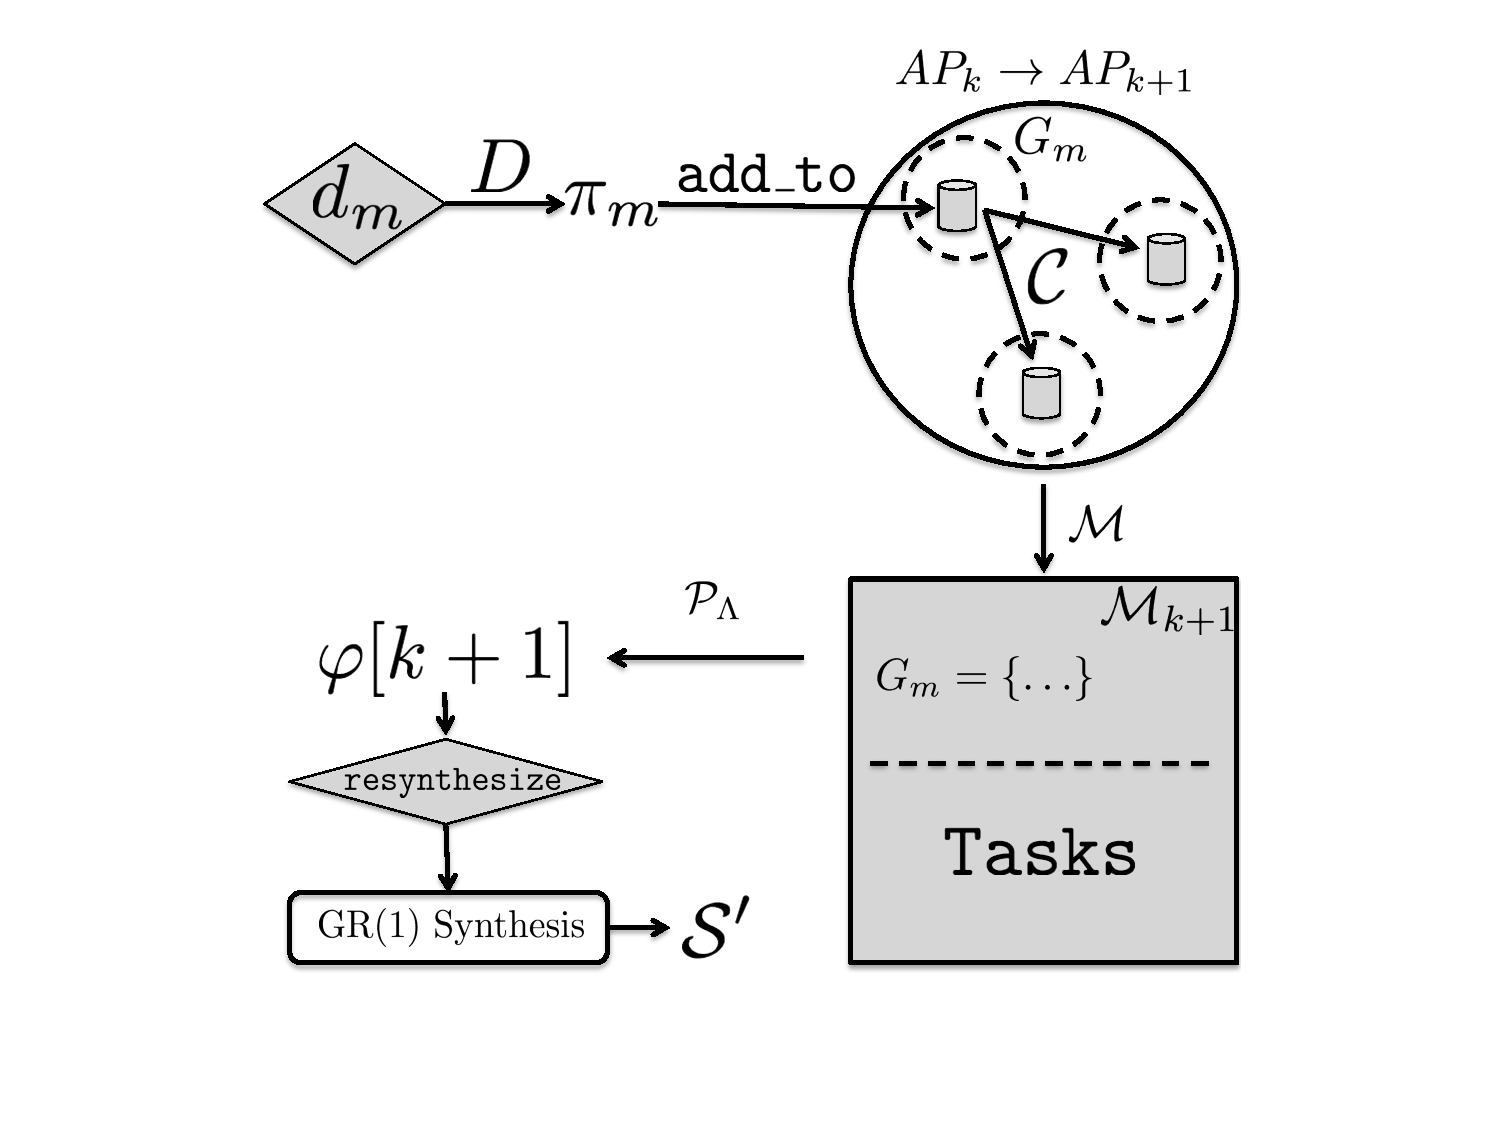
\includegraphics[width=0.9\columnwidth, clip]{./img/approach.pdf}
	\caption{Illustration of our approach, where, for clarity, a single new proposition $\pi_{m}$ is added to a single group $G_m$, which has two corresponding groups $\mathcal{C}(G_m)$. The part of $\mathcal{M}_{k+1}$ denoted as \texttt{Tasks} is immutable throughout the rewriting and resynthesis processes. $\mathcal{S}^\prime$ denotes the revised robot controller.} % TODO: Write stuff here
	\label{Fig:approach}
\end{figure}
% END